\NeedsTeXFormat{LaTeX2e}
\documentclass[14pt,oneside,A4paper,openright]{report}
\usepackage{verbatim}
\usepackage{enumitem}
\usepackage{float}
\usepackage{graphicx}
\usepackage{theorem,amsmath,amssymb,latexsym,amscd,amsxtra}
\usepackage{theorem,amsmath,amssymb,latexsym,amscd,amsxtra,graphicx,graphpap}
\usepackage{mathtools}
\usepackage{pb-diagram}
\usepackage{listings}
\usepackage{color}
%\usepackage{indentfirst}
\usepackage{caption}
%\usepackage{graphicx}
\usepackage{amsmath}
\usepackage{picinpar,floatflt}
\usepackage{ makecell}
\usepackage{longtable}
\usepackage{fancybox}
\usepackage[T1]{fontenc}
\usepackage{array}
\usepackage{multicol}
\usepackage{booktabs}
\usepackage{longtable}
\usepackage[utf8]{vietnam}
\usepackage[tight,vietnam]{minitoc}
\usepackage{anyfontsize}
\usepackage{xpatch}
\usepackage[unicode]{hyperref} % Hỗ trợ nhấp chuột vào trích dẫn
\usepackage{fancyhdr}
\usepackage[left=3.5cm,right=2.0cm,top=3.5cm,bottom=3.0cm, a4paper]{geometry}
%\usepackage{commath}
%==================================
\usepackage{titletoc}
%==================================
\usepackage[numbers,sort&compress]{natbib}
\bibliographystyle{unsrt}
%==================================
\renewcommand{\thechapter}{\arabic{chapter}}
\renewcommand{\thesection}{\arabic{chapter}.\arabic{section}}
\theoremstyle{plain}
\newcommand{\eproof}{\hfill $\square$}
%\newcommand{\eproof}{\hfill}
\newcommand{\chm}{{\bf Chứng minh.}}
\newenvironment{cm}{\chm}{\eproof}
%===============================
\newtheorem{theorem}{Định lý}[section]
\newtheorem{corollary}[theorem]{Hệ quả}
\newtheorem{cy}[theorem]{Chú ý} 
\newtheorem{definition}[theorem]{Định nghĩa}%[section]
\newtheorem{bd}[theorem]{Bổ đề} 
\newtheorem{bt}[theorem]{Bài toán}
\newtheorem{md}[theorem]{Mệnh đề} 
\newtheorem{remark}[theorem]{Nhận xét} 
\newtheorem{Bt}[theorem]{Bài toán} 
\newtheorem{example}[theorem]{Ví dụ} 
\newtheorem{hq}[theorem]{Hệ quả}
\newtheorem{kh}[theorem]{Kí hiệu}
\newtheorem{cor}[theorem]{Hệ quả}
\newtheorem{dfn}[theorem]{Định nghĩa}%[section]
\newtheorem{lem}[theorem]{Bổ đề} 
\newtheorem{prop}[theorem]{Mệnh đề} 
\newtheorem{dl}[theorem]{Định lý}
\newtheorem{vd}[theorem]{\bf Ví dụ} 
\newtheorem{nx}[theorem]{\bf Nhận xét} 
\newtheorem{dn}[theorem]{\bf Định nghĩa} 
\newtheorem{tc}[theorem]{\bf Tính chất} 
\newtheorem{ch}[theorem]{\bf Câu hỏi} 
\newtheorem{ttt}[theorem]{\bf Thuật toán} 
\newtheorem{gt}[theorem]{\bf Giả thiết} 
\renewcommand{\baselinestretch}{1.5}
\setlength{\oddsidemargin}{0.3cm}     %Lề trái tính từ điểm cách mép giấy 2.54cm
\setlength{\topmargin}{-1.75cm}          %Lề trên tính từ điểm cách mép giấy 2.54cm
\setlength{\headsep}{0.75cm}   %Khoang cach tu  Headerline tới Khối chữ
\textwidth=15.5cm
\textheight=24.5cm
\renewcommand{\bibname}{Tài liệu tham khảo}
\renewcommand{\large}{\fontsize{14pt}{14pt}\selectfont}
\renewcommand{\Large}{\fontsize{16pt}{16pt}\selectfont}
\renewcommand{\LARGE}{\fontsize{15pt}{15pt}\selectfont}
\renewcommand{\th}{\fontsize{18pt}{18pt}\selectfont}
\makeatletter
\def\ps@myheadings{
\def\@evenhead{\hfil\thepage\hfil}
\def\@oddhead{
\hfil\thepage\hfil}}
\makeatother
\pagestyle{myheadings}
\definecolor{dkgreen}{rgb}{0,0.6,0}
\definecolor{gray}{rgb}{0.5,0.5,0.5}
\definecolor{mauve}{rgb}{0.58,0,0.82}

\lstset{
    basicstyle=\ttfamily\small,
    numbers=left,
    numberstyle=\tiny\color{gray},
    stepnumber=1,
    numbersep=10pt,
    backgroundcolor=\color[rgb]{0.95,0.95,0.95}, % Màu nền sáng hơn
    showspaces=false,
    showstringspaces=false,
    showtabs=false,
    frame=single, % Có khung bao quanh đoạn code
    rulecolor=\color{black},
    tabsize=2,
    captionpos=b,
    breaklines=true,
    breakatwhitespace=false,
    keywordstyle=\color{blue},
    commentstyle=\color{green},
    stringstyle=\color{red},
}

\lstset{frame=tb,
  language= Python,
  basicstyle={\small\ttfamily},
  aboveskip=3mm,
  belowskip=3mm,
  breakatwhitespace=true,
  breaklines=true,
  classoffset=0,
  columns=flexible,
  commentstyle={\color{dkgreen}, morecomment=[l]{\#}},
  framexleftmargin=0.25em,
  frameshape={}{}{}{},
  keywordstyle=\color{blue},
  numbers=left,
  numberstyle=\tiny\color{gray},
  showstringspaces=false,
  stringstyle=\color{mauve},
  tabsize=3,
  xleftmargin=1em,
}
\newenvironment{proof}{\paragraph{Chứng minh:}}{\hfill$\square$}
\newenvironment{myproof}[2] {\paragraph{Proof of {#1} {#2} :}}{\hfill$\square$}
\DeclarePairedDelimiter{\pro}{\langle}{\rangle}
\DeclarePairedDelimiter{\norm}{\lVert}{\rVert}
\makeatletter
\AtBeginDocument{\xpatchcmd{\@thm}{\thm@headpunct{.}}{\thm@headpunct{}}{}{}}

\fontsize{22pt}{16pt}\selectfont
\begin{document}
\setcounter{page}{1}%
\pagenumbering{roman}

\pagenumbering{gobble}
\begin{center}
\Large
{\bf ĐẠI HỌC BÁCH KHOA HÀ NỘI}\\
{\bf KHOA TOÁN - TIN}
\centerline{--------------------o0o--------------------}  
\end{center}
\vspace{0.3cm}
\begin{figure}[ht]
\begin{center}

\includegraphics[scale=0.6]{dhbkhn.png}\\
\end{center}
\end{figure}
\begin{center}
\fontsize{21pt}{17pt}\selectfont
\vspace{0.35cm}
\textbf{ĐỒ ÁN II}\\
\end{center}

\vspace{0.3cm}
\begin{center}
\fontsize{17pt}{16pt}\selectfont

\bf NGHIÊN CỨU VÀ TRIỂN KHAI QUY TRÌNH CI/CD TRÊN NHIỀU NỀN TẢNG

\end{center}
\vspace{0.3cm}
 \begin{center}
	\fontsize{15pt}{16pt}\selectfont 	
	{\bf Chuyên ngành: TOÁN TIN}\\	
\end{center}

\vspace{0.3cm}
\begin{center}
\begin{tabular}{l l}
\fontsize{13pt}{14pt} \selectfont
Giảng viên hướng dẫn:&\fontsize{13pt}{14pt}{\bf  TS. NGÔ QUỐC HOÀN}\quad $_{\overline{\text{Chữ kí của GVHD}}}$\\[0.5cm]

\fontsize{13pt}{14pt} \selectfont Sinh viên thực hiện:&\fontsize{13pt}{14pt}{\bf TRẦN XUÂN SƠN}\\[0.5cm]

\fontsize{13pt}{14pt} \selectfont {MSSV:}& \fontsize{13pt}{14pt}{\bf 20227149}\\
\end{tabular}

\end{center}
\vspace{2cm}
\begin{center}
\LARGE HÀ NỘI, 10/2025
\end{center}
\newpage
\begin{center}
\fontsize{17pt}{16pt}\selectfont
%\textbf{ĐỒ ÁN TỐT NGHIỆP}\\
\textbf{ĐỒ ÁN II}\\
\end{center}
 \begin{center}
 \vspace{1cm}
\large \bf  Chuyên ngành: Toán Tin\\
\vspace{0.5cm}
%\large	Chuyên sâu: Các phương pháp tối ưu\\
\end{center}

\vspace{3cm}
\begin{center}
\fontsize{17pt}{16pt}\selectfont

\bf  NGHIÊN CỨU VÀ TRIỂN KHAI QUY TRÌNH CI/CD TRÊN NHIỀU NỀN TẢNG

\end{center}

\vspace{3cm}
\begin{center}
\begin{tabular}{l l}
Giảng viên hướng dẫn:&{\bf  TS. NGÔ QUỐC HOÀN}\\[0.5cm]
Họ và tên sinh viên:&{\bf TRẦN XUÂN SƠN}\\[0.5cm]
Mã số sinh viên:&{\bf 20227149}\\[0.5cm]
Lớp:&{\bf      Toán - Tin 02 - K67}
\end{tabular}

\end{center}
\vspace{4cm}
\begin{center}
\LARGE HÀ NỘI, 10/2025
\end{center}

\large

\newpage

\newpage
\thispagestyle{empty}
\thisfancypage{
	\setlength{\fboxsep}{0cm}
	\fbox}{}

\fontsize{22pt}{16pt}\selectfont
\bigbreak
\begin{center}
	{\bf Nhận xét của giảng viên hướng dẫn}
\end{center}
\bigbreak

\fontsize{12pt}{14pt}\selectfont
\begin{enumerate}
	\item [{\bf 1.}]{\bf Mục tiêu và nội dung của đồ án}
	\begin{enumerate}
		\item Mục tiêu: 
		\vspace{40pt}
		\item Nội dung: 
		\vspace{40pt}
	\end{enumerate}
	\item [{\bf 2.}] {\bf Kết quả đạt được} 
	\vspace{60pt}
	\item [{\bf 3.}]{\bf Ý thức làm việc của sinh viên:}
    \vspace{60pt}
\end{enumerate}


\bigskip 
\hspace{7cm}
{\it Hà Nội, ngày .... tháng .... năm ....}

\hspace{7.8cm} {\bf Giảng viên hướng dẫn}

\vspace{2 cm}
%\hspace{7.6cm} {\bf PGS.TS. Nguyễn Đình Hân}



\pagestyle{fancy}
\lhead{ĐỒ ÁN II}
\cfoot{\fontsize{13pt}{18pt} \selectfont \thepage}
\newpage
\begin{center}
\fontsize{22pt}{16pt}\selectfont
{\bfseries Lời cảm ơn}
\fontsize{13pt}{16pt}\selectfont
\end{center}
\bigskip

%Lời đầu tiên, em xin được gửi lời cảm ơn đến thầy cô, gia đình và anh chị em bạn bè xung quanh đã giúp đỡ, ủng hộ em trong suốt quá trình làm Đồ án.
%\bigskip
%
%Cùng với đó, em xin gửi lòng biết ơn sâu sắc đến quý thầy cô Khoa Toán - Tin, Đại học Bách khoa Hà Nội đã dùng tri thức và tâm huyết của mình để có thể truyền đạt cho em những kiến thức quan trọng, quý báu.
%\bigskip
%
%Đặc biệt, em xin gửi lời cảm ơn chân thành đến PGS.TS. Nguyễn Đình Hân người đã tận tâm chỉ bảo, hướng dẫn em trong suốt thời gian làm Đồ án vừa qua. Không chỉ hướng dẫn Đồ án, cô còn là người định hướng con đường học thuật, tạo động lực cho em cố gắng theo đuổi lĩnh vực này.
%\bigskip
%
%Trong quá trình làm Đồ án không thể tránh khỏi những thiếu sót, em rất mong nhận được những ý kiến góp ý của Thầy Cô để Đồ án của em được hoàn thiện hơn.
%\bigskip
%\\
%Em xin chân thành cảm ơn!!

%\begin{minipage}{0.5\textwidth}
%\end{minipage}
%\hspace{0.5\textwidth}
%\begin{minipage}{0.5\textwidth}
%	\noindent\begin{center}
%		\vspace{1cm}
%		\textit{Hà Nội,ngày 13 tháng 6  năm 2025} \\
%		Tác giả đồ án\\ \vspace{2cm}
%		\textbf{Bùi Anh Tú}
%	\end{center}	
%\end{minipage}
%\begin{figure}[H]
%    \centering
%    \includegraphics[width=1\textwidth]{Ảnh/ĐG1.png}
%\end{figure}
%    \includegraphics[width=1\textwidth]{Ảnh/ĐG2.png}
\tableofcontents 
\pagestyle{myheadings}



\newpage


\thispagestyle{empty}
\pagenumbering{arabic}
\setcounter{page}{1}
\newpage
\addcontentsline{toc}{chapter}{\bfseries Danh sách bảng}
\listoftables
%\thispagestyle{empty}
\newpage
\addcontentsline{toc}{chapter}{\bfseries Danh sách hình vẽ}
\listoffigures
\large

\fontsize{12pt}{16pt}\selectfont

\pagestyle{fancy}
\rhead{\leftmark}
\lhead{ĐỒ ÁN II}
\cfoot{\fontsize{13pt}{18pt} \selectfont \thepage}
\chapter*{Ký hiệu và chữ viết tắt}
\addcontentsline{toc}{chapter}{\bfseries Ký hiệu và chữ viết tắt}

\begin{tabular}{@{\hspace{0.5cm}} l @{\hspace{1cm}} p{12cm}}
    CI & Continuous Integration \\
    CD & Continuous Delivery / Continuous Deployment  \\
    DevOps & Development Operations \\
    MTTR & Mean Time To Resolution \\
    RSA & Rivest-Shamir-Adleman \\
    VMs & Virtual Machines \\
%    SHA256 & Secure Hash Algorithm 256-bit \\
%    BFT & Byzantine Fault Tolerance \\
%    ECDSA & Elliptic Curve Digital Signature Algorithm \\
%    BFV & Brakerski/Fan-Vercauteren \\
%    HTTP & Hypertext Transfer Protocol \\
%    API & Application Programming Interface\\
%    ML & Machine Learning\\
%    DPA & Differential Power Analysis\\
%    EM & Electromagnetic Attack\\
\end{tabular}
\chapter*{Tóm tắt nội dung}
%\addcontentsline{toc}{chapter}{Tóm tắt nội dung}
%Nội dung đồ án nghiên cứu và xây dựng quy trình CI/CD trên nhiều nền tảng khác nhau. Được phát triển dựa trên mô hình được đưa ra trong một bài báo công bố khoa học \textit{Privacy preserving verifiable federated learning scheme using blockchain and homomorphic encryption} \cite{1.3} được công bố trong cuộc thi \textit{Applied Soft Computing 167}. Bài báo này giới thiệu một mô hình học liên kết có thể xác minh và bảo vệ quyền riêng tư mới (PPVFL – Privacy-Preserving Verifiable Federated Learning) tích hợp công nghệ blockchain và mã hóa đồng hình (homomorphic encryption) nhằm giải quyết các thách thức quan trọng trong học máy. Mô hình đề xuất đảm bảo quyền riêng tư dữ liệu, tính toàn vẹn, khả năng xác minh, bảo mật mạnh mẽ và hiệu quả trong việc bảo vệ quyền riêng tư của người dùng.
%
%\vfill
%\begin{tabular}{c c}
%      \hspace{6.5cm}  &  \textit{Hà Nội, ngày 13 tháng 06 năm 2025}\\
%       &Sinh viên\\
%       \vspace{2cm}\\
%       & \textbf{Bùi Anh Tú}
%\end{tabular}
%\vfill

\chapter*{Mở đầu}
\addcontentsline{toc}{chapter}{Mở đầu}

Trong kỷ nguyên chuyển đổi số, nơi tốc độ phát triển và chất lượng sản phẩm là yếu tố sống còn, khả năng triển khai phần mềm nhanh chóng, liên tục và đáng tin cậy đã trở thành ưu tiên hàng đầu của mọi tổ chức. Phương pháp phát triển truyền thống với các quy trình tích hợp và phân phối thủ công không còn đáp ứng được yêu cầu về tốc độ thị trường. Chính vì vậy, Tích hợp Liên tục và Phân phối/Triển khai Liên tục (CI/CD) đã nổi lên như một giải pháp kỹ thuật cốt lõi.

Về mặt lịch sử, khái niệm Tích hợp Liên tục (CI) được giới thiệu lần đầu tiên bởi Grady Booch vào năm 1991, nhưng đã được phổ biến rộng rãi và đưa vào thực tiễn phát triển phần mềm hiện đại bởi Kent Beck vào cuối những năm 1990. Tiếp nối CI, khái niệm Phân phối Liên tục (Continuous Delivery – CD) đã được hệ thống hóa và làm rõ trong cuốn sách cùng tên (xuất bản năm 2010) của Jez Humble và David Farley, trở thành nền tảng quan trọng trong văn hóa DevOps ngày nay.

CI/CD tự động hóa toàn bộ vòng đời phát triển phần mềm, từ khi các lập trình viên tích hợp mã nguồn (CI) đến khi ứng dụng được chuyển giao hoặc triển khai tới môi trường sản xuất (CD). Tầm quan trọng của CI/CD được chứng minh rõ rệt qua các số liệu: theo khảo sát của GitLab (2024), các nhóm phát triển phần mềm áp dụng CI/CD cho thấy tỷ lệ thành công khi triển khai tăng 42\% so với các nhóm không áp dụng phương pháp này, đồng thời giúp giảm thiểu đáng kể thời gian xử lý lỗi (MTTR), một chỉ số then chốt về khả năng bảo trì hệ thống. Báo cáo đồ án 2 sẽ đi sâu vào nghiên cứu và triển khai quy trình CI/CD trên nhiều nền tảng. 
%Chúng tôi sẽ đánh giá các chiến lược và công cụ cần thiết để duy trì tính nhất quán, hiệu suất và bảo mật cho pipeline CI/CD khi triển khai các ứng dụng trên các môi trường đa dạng, từ hạ tầng đám mây (Cloud) đến các hệ thống vật lý (On-premise) hay nền tảng di động (Mobile).

%Nguồn tham khảo số liệu/lịch sử:
%
%Grady Booch & Kent Beck: Nguồn gốc của Continuous Integration (CI).
%
%Jez Humble & David Farley: Tác giả cuốn sách "Continuous Delivery" (2010), hệ thống hóa Continuous Delivery (CD).
%
%Tỷ lệ thành công khi triển khai tăng 42\%: Thống kê từ GitLab (theo báo cáo/nghiên cứu về CI/CD).
%
%Giảm thiểu thời gian xử lý lỗi (MTTR): Lợi ích cốt lõi được công nhận rộng rãi của CI/CD (Tham khảo các tài liệu và nghiên cứu về DevOps/CI/CD).

Nội dung đồ án 2 được tổ chức thành các chương sau:

\begin{itemize}
	\item Chương 1. Giới thiệu chung: Trình bày tổng quát về CI/CD (Tích hợp và Phân phối/Triển khai Liên tục), bao gồm khái niệm, ưu điểm, hạn chế, và cách thức hoạt động cơ bản của quy trình.
	
	\item Chương 2. Giới thiệu các nền tảng và công cụ triển khai CI/CD: Giới thiệu và so sánh các nền tảng CI/CD cốt lõi được sử dụng: GitHub, GitLab, và Jenkins. Đồng thời, giới thiệu các công cụ hỗ trợ cần thiết khác như VMware Workstation Pro, Nginx, và SonarQube.
	
	\item Chương 3. Xây dựng hệ thống server ảo: Trình bày chi tiết việc xây dựng môi trường server ảo (VMs) và mô tả Kiến trúc hệ thống cụ thể cho việc triển khai CI/CD trên từng nền tảng (GitHub, GitLab và Jenkins).
	
	\item Chương 4. Xây dựng và triển khai quy trình CI/CD: Tập trung vào các bước thực hiện trọng tâm: Xây dựng quy trình CI/CD cho ứng dụng mẫu và tiến hành triển khai quy trình trên các môi trường đã thiết lập.
	
	\item Chương 5. Xây dựng các trường hợp kiểm thử và trình bày kết quả: Trình bày việc xây dựng các trường hợp kiểm thử và phân tích kết quả kiểm thử tự động, đánh giá hiệu quả của quy trình CI/CD đa nền tảng.
	
	\item Kết luận và hướng nghiên cứu: Tổng kết kết quả đạt được và đề xuất hướng cải thiện hoặc mở rộng nghiên cứu trong tương lai.
\end{itemize}




\chapter{Giới thiệu chung}

\section{Đặt vấn đề}
Trong các doanh nghiệp, các các lập trình viên chịu trách nhiệm viết code cho dự án, còn các kỹ sư vận hàng và triển khai hạ tầng đảm nhận việc lấy mã nguồn và triển khai. Khi chỉ có một hoặc hai mã nguồn, việc triển khai chưa quá phức tạp. Tuy nhiên, thực tế một doanh nghiệp có thể có hàng chục, thậm chí hàng trăm mã nguồn. Chỉ riêng với 20 dự án trên \textbf{Git}, đã đặt ra câu hỏi: cần bao nhiêu kỹ sư vận hàng và triển khai hạ tầng để triển khai kịp tiến độ?
Quá trình phát triển dự án thường diễn ra trên ba môi trường chính:
\begin{itemize}
	\item \textbf{Development}: Môi trường để lập trình viên cập nhật các đoạn mã nguồn mới
	\item \textbf{Staging}: Môi trường kiểm thử, đảm bảo mọi thứ chạy ổn trước khi lên production và thường được các tester sử dụng.
	\item \textbf{Production}: Môi trường phục vụ người dùng cuối.
\end{itemize}



Trong môi trường \textbf{Development}, các lập trình viên cập nhật mã nguồn  hàng giờ, thậm chí hàng phút, và họ cần kiểm tra mã nguồn trên môi trường kiểm thử trước khi chuyển sang các môi trường quan trọng hơn. Nếu phải chờ các kỹ sư triển khai thủ công, điều này sẽ rất tốn thời gian và ảnh hưởng đến hiệu suất dự án.
Không chỉ lập trình viên gặp khó khăn, đội ngũ vận hàng và triển khai cũng gặp nhiều trở ngại khi triển khai thủ công: sao chép mã nguồn giữa các máy chủ có thể dẫn đến sai sót; họ phải truy cập từng máy chủ, \textbf{clone} mã nguồn, \textbf{build}, \textbf{run}, rồi kiểm tra \textbf{logs}… Ngoài ra, triển khai dự án còn bao gồm nhiều công việc khác như cài đặt hệ thống, giám sát, bảo trì và nâng cấp, làm quá trình triển khai trở nên phức tạp và tốn thời gian.

\section{Khái niệm CI/CD}

\begin{figure}[htbp]
	\centering
	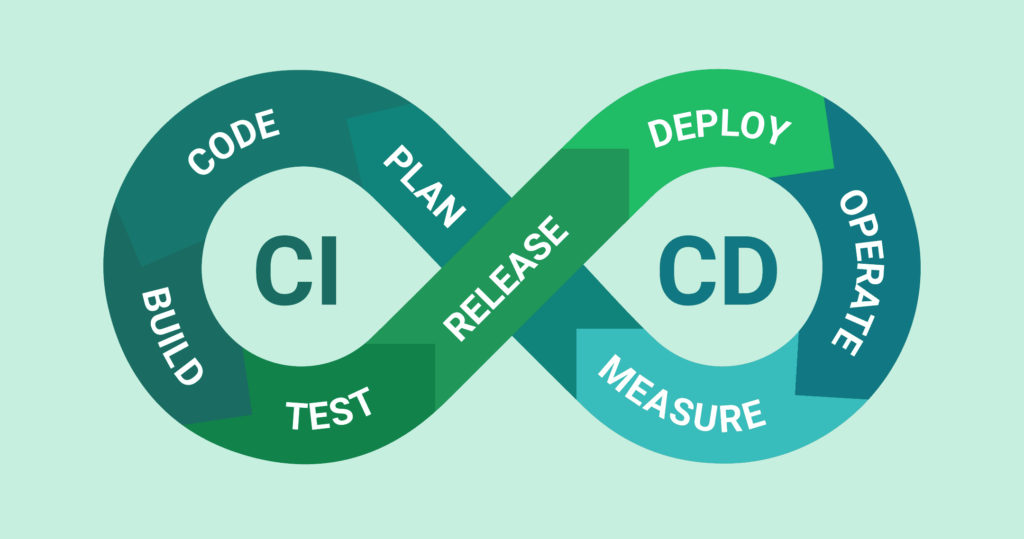
\includegraphics[width=1\linewidth]{Ảnh/defination-ci-cd.png}
	\caption{Mô Hình CI/CD}
	\label{fig:Mô Hình CI/CD}
\end{figure}


Để giải quyết các khó khăn trong phần trên, \textbf{CI/CD} ra đời.\textbf{ CI/CD} gồm hai phần chính:



\subsection*{CI (Continuous Integration)}

Bước CI bao gồm: clone mã nguồn, build dự án, và tích hợp các bước kiểm thử như:
\begin{enumerate}
	\item Kiểm tra hiệu năng 
	\item Kiểm tra chất lượng mã nguồn
	\item Kiểm tra bảo mật
	\item Và nhiều loại kiểm thử khác
\end{enumerate}
Mục tiêu là đảm bảo chất lượng mã nguồn trước khi triển khai.

\subsection*{CD (Continuous Deployment / Continuous Delivery)}
\begin{itemize}
	\item \textbf{Continuous Deployment}: triển khai hoàn toàn tự động. Lập trình viên chỉ cần commit code, chức năng mới sẽ được triển khai ngay mà không cần thao tác thủ công.
	\item \textbf{Continuous Delivery}: triển khai vẫn yêu cầu bước xác nhận thủ công. Code sau khi \textbf{build} và kiểm thử chỉ được triển khai khi có sự đồng ý từ team.
\end{itemize}



Mỗi chiến lược \textbf{CD} có ưu nhược điểm riêng:
\begin{itemize}[label=\textendash] 
	\item 	Triển khai tự động tối ưu hiệu suất và rút ngắn thời gian ra môi trường thực tế.
	\item Triển khai thủ công giúp tăng khả năng kiểm soát, giảm rủi ro lỗi khi đưa code vào môi trường quan trọng.
	Tùy theo nhu cầu doanh nghiệp, có thể kết hợp cả hai để xây dựng quy trình \textbf{CI/CD} tối ưu, vừa nhanh, vừa an toàn.
\end{itemize}


\section{Ưu điểm và hạn chế của quy trình CI/CD}

\subsection*{Ưu điểm}

	Việc triển khai quy trình \textbf{CI/CD} mang lại nhiều lợi ích rõ rệt cho đội ngũ phát triển phần mềm:

\begin{enumerate}
	\item \textbf{Giảm thiểu lỗi không đáng có:}  
	Nhờ có CI/CD, các lỗi như lỗi biên dịch hoặc lỗi phát sinh do khác biệt môi trường build được phát hiện sớm.  
	Ví dụ: cùng một source code nhưng khi bạn A build trên máy của mình và bạn B build trên máy khác có thể cho ra kết quả khác nhau.  
	Với \textbf{CI/CD}, tất cả đều được build trong môi trường thống nhất, giúp loại bỏ rủi ro này.
	
	\item \textbf{Đảm bảo tính ổn định và logic của hệ thống:}  
	Các bài kiểm thử tự động giúp bảo đảm rằng việc thêm tính năng mới không ảnh hưởng đến các chức năng hiện có.
	
	\item \textbf{Tăng hiệu quả làm việc:}  
	Kỹ sư vận hành và hạ tầng không cần tự build hay deploy ứng dụng nữa, vì mọi thao tác đã được tự động hóa.  
	Điều này giúp họ tập trung hơn vào việc phát triển và cải thiện chất lượng phần mềm.
	
	\item \textbf{Nâng cao chất lượng mã nguồn:}  
	CI/CD cho phép thiết lập các quy tắc ngay từ đầu, chẳng hạn như giới hạn kích thước của pull request hoặc số lượng thay đổi tối đa.  
	Nhờ vậy, quy trình đánh giá mã nguồn trở nên rõ ràng và chất lượng mã nguồn được cải thiện.
	
	\item \textbf{Phát triển kỹ năng viết Unit Test:}  
	Khi pipeline có chỉ số ràng buộc về \textit{code coverage}, Developer cần đảm bảo phần code mới có đủ kiểm thử để không làm giảm tỷ lệ bao phủ.  
	Điều này giúp các developer hình thành thói quen viết Unit Test và nâng cao kỹ năng kiểm thử tự động.
	
	\item \textbf{Tối ưu tốc độ phát triển sản phẩm:}  
	CI/CD cho phép theo dõi chi tiết thời gian build, test hay lint check, giúp nhóm phát triển dễ dàng phát hiện và tối ưu các khâu còn chậm.
\end{enumerate}

\subsection*{Hạn chế}

Bên cạnh những ưu điểm nổi bật, CI/CD cũng có một số hạn chế cần lưu ý:

\begin{enumerate}
	\item \textbf{Xung đột khi nhiều lập trình viên cùng làm việc:}  
	Khi có nhiều pull request cần merge vào branch, pipeline có thể bị tắc nghẽn.  
	Các thành viên phải chờ người khác merge xong, sau đó cập nhật lại code nếu có conflict và chạy test lại từ đầu, gây gián đoạn quá trình phát triển.
	
	\item \textbf{Phụ thuộc vào dịch vụ bên thứ ba:}  
	Nếu tổ chức sử dụng nền tảng CI/CD của bên ngoài như Jenkins Cloud, GitLab CI hoặc GitHub Actions,  
	khi dịch vụ gặp sự cố hoặc ngừng hoạt động, toàn bộ pipeline sẽ bị ảnh hưởng, làm gián đoạn quá trình phát triển phần mềm.
\end{enumerate}


\section{Cách thức hoạt động của quy trình CI/CD}

\begin{figure}[htbp]
	\centering
	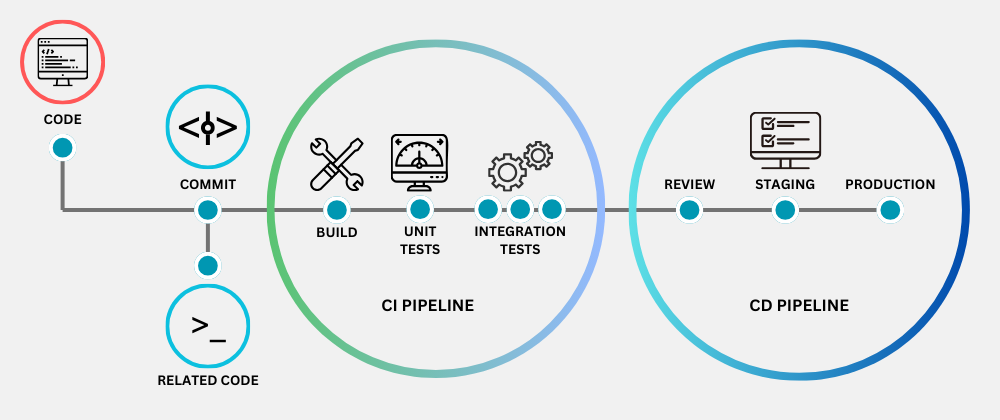
\includegraphics[width=1\linewidth]{Ảnh/ci-cd-pipeline.png}
	\caption{Quy trình CI/CD}
	\label{fig:Quy trình CI/CD}
\end{figure}


Quy trình CI/CD được vận hành thông qua sự phối hợp giữa hai thành phần chính:
\begin{enumerate}
	\item \textbf{Git Repository} – nơi lưu trữ mã nguồn và quản lý toàn bộ thay đổi trong dự án.
	\item \textbf{CI/CD Tool} – công cụ đảm nhiệm việc tự động hóa các giai đoạn như build, test, deploy và theo dõi kết quả.
\end{enumerate}

Cụ thể, khi một Developer thực hiện thay đổi trong Git repository (ví dụ: tạo \textit{pull request} hoặc \textit{commit} mới), Git sẽ gửi thông báo đến CI/CD tool rằng có cập nhật mới được tạo. Ngay sau đó, CI/CD tool tự động kích hoạt pipeline và chạy tuần tự các bước đã được cấu hình sẵn, thường bao gồm:

\begin{itemize}
	\item \textbf{Biên dịch mã nguồn (Build):} Toàn bộ mã nguồn được biên dịch để kiểm tra tính hợp lệ, đảm bảo không có lỗi cú pháp hoặc lỗi phụ thuộc thư viện.
	\item \textbf{Kiểm thử tự động (Testing):} Hệ thống thực hiện các bài kiểm thử đơn vị (unit test), kiểm thử tích hợp (integration test), hoặc kiểm thử giao diện (UI test) để đảm bảo logic chương trình hoạt động đúng.
	\item \textbf{Phân tích chất lượng mã (Static Code Analysis):} Mã nguồn được kiểm tra bằng các công cụ như SonarQube, ESLint hoặc Checkstyle để phát hiện lỗi tiềm ẩn, vi phạm quy tắc code, hoặc các rủi ro bảo mật.
	\item \textbf{Kiểm tra quy tắc (Code Policy Check):} Pipeline xác minh các quy định nội bộ như kích thước \textit{pull request}, quy ước đặt tên, hay tiêu chuẩn lập trình.
\end{itemize}

\subsection*{Giai đoạn sau kiểm thử (Post-testing stage)}

Khi toàn bộ các bài kiểm thử và kiểm tra chất lượng mã đều đạt yêu cầu, CI/CD tool sẽ tự động chuyển sang các bước xử lý tiếp theo:

\begin{enumerate}
	\item \textbf{Đóng gói và build artifact:}  
	Mã nguồn sau khi được xác nhận hợp lệ sẽ được đóng gói thành một \textit{artifact} (ví dụ: file \texttt{.jar}, \texttt{.war}, \texttt{.zip} hoặc Docker image).  
	Artifact này được lưu trữ trong kho lưu trữ riêng (như Artifactory, Nexus hoặc Docker Registry) để phục vụ cho việc triển khai ở các môi trường tiếp theo.
	
	\item \textbf{Triển khai tự động (Deploy):}  
	Hệ thống tự động triển khai artifact vừa build lên môi trường \textit{staging} hoặc \textit{production} tùy theo cấu hình.  
	Việc deploy có thể được thực hiện thông qua các công cụ như Jenkins, GitLab CI/CD, ArgoCD hoặc Kubernetes.  
	Ở giai đoạn này, pipeline có thể tích hợp thêm các bài kiểm thử sau triển khai (post-deployment tests) nhằm xác nhận ứng dụng hoạt động đúng trên môi trường thực tế.

	
	\item \textbf{Khả năng rollback:}  
	Trong trường hợp phiên bản mới gây lỗi hoặc ảnh hưởng đến hệ thống, pipeline hỗ trợ cơ chế \textbf{rollback} để quay lại phiên bản ổn định trước đó.  
	Rollback có thể được thực hiện thủ công hoặc tự động (auto-rollback) nếu hệ thống phát hiện các chỉ số bất thường như downtime, lỗi 5xx, hoặc giảm hiệu năng.
\end{enumerate}

\subsection*{Tổng kết}

Khi toàn bộ quá trình hoàn tất, CI/CD tool phản hồi kết quả ngược lại cho Git repository, thể hiện trạng thái của \textit{pull request} hoặc \textit{commit} là thành công hoặc thất bại.  
Dựa vào đó, tester có thể dễ dàng đánh giá sơ bộ chất lượng code trước khi thực hiện đánh giá chi tiết.

Tuy nhiên, quy trình CI/CD chỉ có thể tự động hóa và kiểm soát được một phần logic kỹ thuật.  
Việc đánh code thủ công từ lập trình viên hoặc tester vẫn là bước cần thiết nhằm đảm bảo mã nguồn đáp ứng tiêu chuẩn của nhóm và xử lý được những trường hợp logic phức tạp mà hệ thống tự động chưa thể bao quát hết.



\chapter{Giới thiệu các nền tảng và ông cụ triển khai CI/CD}


\section{Các nền tảng được sử dụng triển khai CI/CD}

Để triển khai một quy trình CI/CD hiệu quả thì có rất nhiều yếu tố phải quan tâm như là: Những tài nguyên hiện có của dự án, kinh nghiệm sử dụng các công cụ của các kỹ sư trong công ty và chi phí để phát triển dự án, ... Và từ những yếu tố khác nhau đó thì mỗi dữ án, mỗi công ty sẽ phải lựa chọn những nền tảng và công cụ phù hợp để xây dựng quy trình CI/CD của mình. Hiện nay, ba nền tảng phổ biến thường được sử dụng là GitHub, GitLab và Jenkins, mỗi nền tảng có đặc điểm và cách tiếp cận riêng, phù hợp với những nhu cầu khác nhau của dự án. 

\subsection{GitHub}

GitHub là nền tảng quản lý mã nguồn phổ biến, nổi bật với sự đơn giản, dễ sử dụng và tích hợp mạnh mẽ với nhiều công cụ bên thứ ba. GitHub hỗ trợ quản lý phiên bản, theo dõi lịch sử thay đổi, và cung cấp môi trường cộng tác trực tuyến, giúp các nhóm phát triển dễ dàng làm việc cùng nhau.

\subsubsection{GitHub Cloud}
GitHub Cloud là dịch vụ lưu trữ mã nguồn trên đám mây, giúp người dùng truy cập dự án từ bất kỳ đâu mà không cần cài đặt và quản lý server riêng. Nhờ GitHub Cloud, các dự án nhỏ hoặc các nhóm làm việc phân tán có thể triển khai CI/CD nhanh chóng, tận dụng hạ tầng sẵn có của GitHub. Ngoài ra, GitHub Cloud luôn được cập nhật và bảo mật bởi chính đội ngũ GitHub, giúp giảm gánh nặng vận hành cho doanh nghiệp.

\subsubsection{GitHub Actions}
GitHub Actions là công cụ tích hợp sẵn cho phép tự động hóa workflow CI/CD trực tiếp trên GitHub. Actions cho phép cấu hình các pipeline để tự động build, test, deploy mỗi khi có thay đổi trong kho mã nguồn. GitHub Actions hỗ trợ nhiều môi trường, từ Linux, Windows, macOS đến các container, đồng thời có thư viện hành động (actions) phong phú giúp triển khai nhanh chóng mà không cần viết script phức tạp. Nhờ đó, GitHub trở thành nền tảng CI/CD “all-in-one” tiện lợi cho các dự án vừa và nhỏ.

\subsection{GitLab}

GitLab là nền tảng quản lý mã nguồn toàn diện, nổi bật với khả năng kết hợp quản lý dự án, issue tracking và CI/CD trong cùng một hệ sinh thái. GitLab phù hợp với các tổ chức muốn kiểm soát toàn bộ vòng đời phát triển phần mềm từ một nơi, từ lập kế hoạch, phát triển, kiểm thử đến triển khai.

\subsubsection{GitLab Server}
GitLab Server có thể được cài đặt trên máy chủ riêng hoặc trên cloud do tổ chức quản lý. Nó cung cấp toàn quyền kiểm soát về bảo mật, truy cập và cấu hình pipeline CI/CD, đồng thời hỗ trợ quản lý các dự án lớn với nhiều nhóm phát triển. GitLab Server đặc biệt phù hợp cho các doanh nghiệp có yêu cầu cao về bảo mật hoặc muốn duy trì dữ liệu nội bộ.

\subsubsection{GitLab Runner}
GitLab Runner là thành phần thực thi các công việc CI/CD, chịu trách nhiệm build, test và deploy theo pipeline đã cấu hình. Runner có thể được cài đặt trên nhiều máy, giúp phân tán tải và tăng tốc độ xử lý pipeline. GitLab Runner cũng linh hoạt về môi trường triển khai, có thể chạy trong container, máy vật lý hoặc cloud, cho phép tùy chỉnh theo nhu cầu cụ thể của từng dự án. Nhờ vậy, GitLab vừa cung cấp khả năng kiểm soát nội bộ, vừa hỗ trợ tự động hóa CI/CD hiệu quả.

\subsection{Jenkins}

Jenkins là một công cụ tự động hóa mã nguồn mở, nổi bật với khả năng linh hoạt, plugin phong phú và hỗ trợ tích hợp với hầu hết các hệ thống hiện có. Jenkins phù hợp với các dự án cần pipeline CI/CD phức tạp, với nhiều bước kiểm thử, build, deploy và các quy trình tùy chỉnh đặc thù.

\subsubsection{Jenkins Server}
Jenkins Server là trung tâm quản lý, nơi lưu trữ cấu hình pipeline, trigger build khi có thay đổi trong kho mã nguồn và tổng hợp kết quả thực thi từ các agent. Server chịu trách nhiệm điều phối workflow CI/CD, cung cấp giao diện quản lý trực quan và báo cáo kết quả các pipeline. Jenkins Server thường được cài đặt trên máy chủ riêng hoặc máy chủ cloud, và có thể mở rộng quy mô bằng cách thêm nhiều agent để thực thi pipeline.

\subsubsection{Jenkins Agent}
Jenkins Agent thực hiện các công việc build, test, deploy theo chỉ định của Jenkins Server. Agent giúp phân tán tải, chạy pipeline trên nhiều môi trường khác nhau, từ Linux, Windows, macOS đến các container. Nhờ Agent, Jenkins có thể xử lý các pipeline phức tạp, hỗ trợ nhiều dự án cùng lúc và tối ưu hiệu suất hệ thống. Cấu trúc Server-Agent của Jenkins cũng cho phép mở rộng linh hoạt, thích hợp cho các dự án lớn hoặc doanh nghiệp có nhiều nhóm phát triển.

\subsection{So sánh ba nền tảng Github, Gitlab, Jenkins}

\begin{itemize}
	\item GitHub phù hợp với các dự án nhỏ và vừa, ưu điểm là dễ sử dụng, nhanh chóng triển khai CI/CD mà không cần hạ tầng riêng. Tuy nhiên đối với các dự án đòi hỏi tính bảo mật cao thì việc công khai mã nguồn dụ án của mình trên Github cloud là điều thể. Nếu sử dụng các dịch vụ cho doanh nghiệp của Github để triển khai dự án thì chi phí quá cao. Vì vậy, Github phù hợp các dự án nhỏ và không đòi hỏi bảo mật cao.
	\item GitLab thích hợp với doanh nghiệp muốn kiểm soát toàn bộ vòng đời phát triển, đặc biệt khi cần cài đặt trên server nội bộ. Gitlab hỗ trợ  cài đặt Gitlab server trên máy chủ của công ty tăng tính bảo mật, so với Github thì gitlab cung cấp nhiều bộ công cụ hơn, nhiều tính năng cho dự án lớn. Đây là cũng là công cụ thường được các doanh nghiệp sử dụng.
	\item Jenkins mạnh về linh hoạt và khả năng mở rộng, phù hợp với các pipeline phức tạp và dự án lớn, nhưng yêu cầu vận hành nhiều hơn. So với 2 nền tảng trước Jenkins là nên tảng mạnh mã nhất về triển khai tự động, cho kỹ sư vận hàng những khả năng tùy biến cao. Tuy không trực tiếp lưu trữ mã nguồn, nhưng với việc tích hợp được nhiều tiện ích đã khiến Jenkins được nhiều công ty lớn tin dùng. Tuy vậy, Jenkins là nền tảng phức tạp đòi hỏi đội ngũ vận hành phải học thêm kỹ năng để sử dụng.
\end{itemize}

Nhờ những đặc điểm này, việc lựa chọn nền tảng CI/CD phụ thuộc vào quy mô dự án, yêu cầu bảo mật, ngân sách và mức độ phức tạp của pipeline.

\section{Các công cụ và ứng dụng cần thiết khác}

Ngoài các nền tảng CI/CD chính, quá trình triển khai phần mềm còn cần một số công cụ hỗ trợ khác để đảm bảo môi trường phát triển, quản lý server và kiểm soát chất lượng mã nguồn. Các công cụ này giúp tăng tính ổn định, tối ưu hóa hiệu suất và đảm bảo phần mềm luôn đạt chất lượng cao trước khi triển khai.

\subsection{VMware Workstation Pro}

VMware Workstation Pro là phần mềm ảo hóa mạnh mẽ, cho phép tạo và quản lý nhiều máy ảo trên cùng một máy tính vật lý. Trong quá trình phát triển và triển khai CI/CD, VMware Workstation Pro giúp: 
\begin{itemize} 
	\item Tạo môi trường thử nghiệm giống hệt môi trường thực tế mà không ảnh hưởng đến máy chủ chính. 
	\item Chạy nhiều hệ điều hành khác nhau song song, thuận tiện cho việc kiểm thử đa nền tảng. 
	\item Dễ dàng sao lưu, khôi phục máy ảo, giảm thiểu rủi ro khi triển khai thử nghiệm.
\end{itemize}

Nhờ VMware Workstation Pro, các nhóm phát triển có thể mô phỏng môi trường triển khai, kiểm tra tính tương thích và đảm bảo các pipeline CI/CD hoạt động ổn định trước khi đưa phần mềm lên server thật.

\subsection{Nginx}

Nginx là một web server và reverse proxy phổ biến, nổi bật với khả năng xử lý lượng lớn kết nối đồng thời và hiệu suất cao. Trong quy trình CI/CD, Nginx thường được sử dụng để: 
\begin{itemize} 
	\item Phục vụ ứng dụng web sau khi deploy, đảm bảo tốc độ tải trang nhanh và ổn định. 
	\item Reverse proxy để điều phối các request đến nhiều server backend khác nhau, hỗ trợ triển khai microservices. 
	\item Cấu hình SSL/TLS để bảo mật kết nối giữa client và server. 
\end{itemize}

Nginx giúp đảm bảo rằng các ứng dụng được triển khai thông qua pipeline CI/CD có thể hoạt động mượt mà trong môi trường sản xuất, đồng thời hỗ trợ các chiến lược deploy như blue-green hoặc canary deployment.

\subsection{SonarQube}

SonarQube là công cụ phân tích chất lượng mã nguồn tự động, hỗ trợ phát hiện lỗi, code smells và các vấn đề về bảo mật ngay trong giai đoạn phát triển. Khi tích hợp vào CI/CD, SonarQube giúp: 
\begin{itemize} 
	\item Phân tích mã nguồn sau mỗi lần commit hoặc build, đảm bảo chất lượng code được duy trì. 
	\item Đưa ra báo cáo chi tiết về lỗi tiềm ẩn, các tiêu chuẩn coding và khả năng bảo mật. 
	\item Hỗ trợ nhiều ngôn ngữ lập trình, dễ dàng tích hợp với các nền tảng CI/CD như GitHub Actions, GitLab CI/CD hay Jenkins. 
\end{itemize}

Việc sử dụng SonarQube trong pipeline CI/CD giúp nâng cao chất lượng phần mềm, giảm thiểu lỗi sản phẩm và đảm bảo code luôn tuân thủ các chuẩn mực kỹ thuật.

\subsection{Docker}

Docker là nền tảng mã nguồn mở cho phép đóng gói, triển khai và chạy ứng dụng trong các container — môi trường nhẹ, độc lập và nhất quán giữa các hệ thống.  
Khi tích hợp vào quy trình CI/CD, Docker mang lại nhiều lợi ích quan trọng như:

\begin{itemize}
	\item Giúp tạo môi trường triển khai đồng nhất giữa các giai đoạn (phát triển, kiểm thử, sản xuất), hạn chế lỗi do khác biệt cấu hình.
	\item Tăng tốc độ triển khai nhờ cơ chế container hóa, cho phép khởi tạo và hủy môi trường chỉ trong vài giây.
	\item Dễ dàng tích hợp với các hệ thống CI/CD như Jenkins, GitHub Actions hay GitLab CI/CD để tự động hóa quá trình build và deploy ứng dụng.
	\item Cho phép quản lý phiên bản của môi trường chạy thông qua Dockerfile, giúp đảm bảo tính tái lập và kiểm soát thay đổi.
\end{itemize}

Việc sử dụng Docker trong pipeline CI/CD giúp đảm bảo quá trình triển khai nhanh chóng, ổn định và dễ mở rộng, đồng thời giảm thiểu các rủi ro khi triển khai ứng dụng trên nhiều môi trường khác nhau.


\chapter{Xây dựng hệ thống server ảo}

\section {Giới thiệu kiến trúc hệ thống}

\subsection{Kiến trúc sử dụng cho nền tảng Github và Gitlab}
%\begin{figure}[htbp]
%	\centering
%	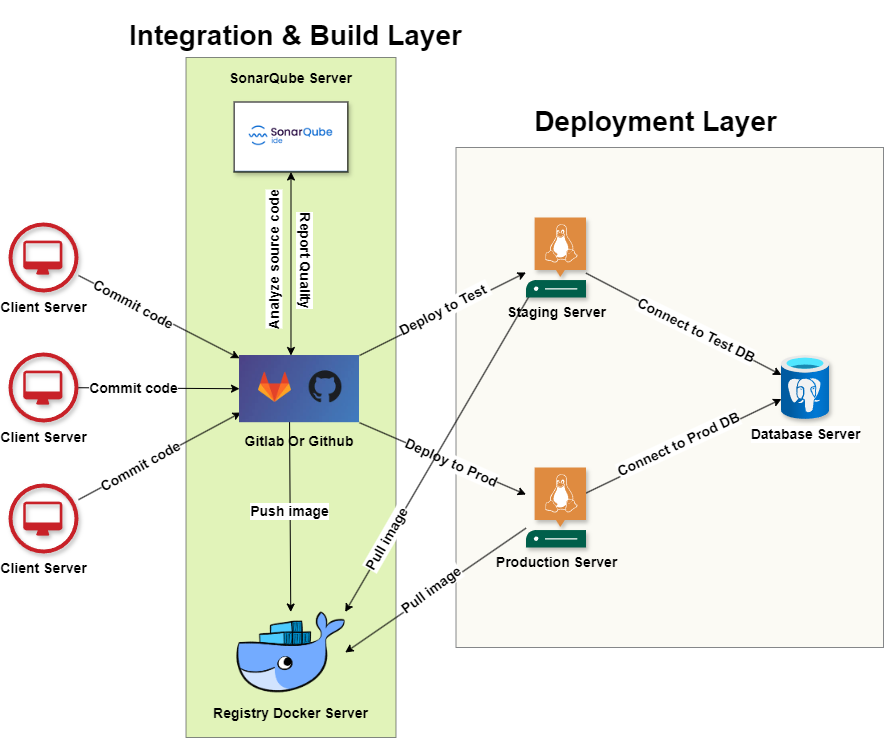
\includegraphics[width=1\linewidth]{Ảnh/gitlab-github-system-achitecture.png}
%	\caption{Kiến trúc hệ thống cho Gitlab và Github}
%	\label{fig:gitlab-github-system-achitecture}
%\end{figure}
%
%Hệ thống trên triển khai sử dụng hai nền tảng quản lý mã nguồn phổ biến là \textbf{GitHub} và \textbf{GitLab}, trong đó GitHub sử dụng \textbf{GitHub Cloud}, còn GitLab được cài đặt dưới dạng \textbf{GitLab Server} nội bộ trên hệ thống ảo. 
%
%
%Ở phía ngoài cùng bên trái của Hình~\ref{fig:gitlab-github-system-achitecture} là các máy khách (client).
%Các máy khách này do các lập trình viên (developer) sử dụng để phát triển phần mềm và thực hiện các thao tác như \textbf{pull/push} mã nguồn lên các nền tảng lưu trữ như GitHub hoặc GitLab.
%Việc kết nối giữa máy khách và máy chủ được thực hiện thông qua các \textbf{giao thức bảo mật SSH hoặc HTTPS}, giúp đảm bảo tính an toàn và xác thực khi truyền tải dữ liệu mã nguồn.
%
%
%Kiến trúc chính của hệ thống được chia thành hai lớp: \textbf{Integration \& Build Layer} và \textbf{Deployment Layer}, với các máy chủ được cấu hình và kết nối như Hình~\ref{fig:gitlab-github-system-achitecture}.
%
%\subsubsection*{Integration \& Build Layer}
%
%Lớp này là trung tâm của quá trình phát triển và kiểm thử phần mềm. 
%Nó bao gồm các máy chủ và dịch vụ chịu trách nhiệm lưu trữ mã nguồn, kiểm tra chất lượng, và đóng gói ứng dụng.
%\begin{itemize}
%	\item GitHub Cloud/ GitLab Server
%	
%	Hai máy chủ này đóng vai trò là \textbf{trung tâm quản lý mã nguồn}. Toàn bộ mã được lưu trữ và quản lý theo từng nhánh (\textit{branch}) hoặc phiên bản (\textit{commit}). 
%	
%	\begin{itemize}
%		\item Đối với \textbf{GitLab}, hệ thống được \textbf{cài đặt trên máy ảo nội bộ} (VMWare Workstation Pro), giúp nhóm phát triển kiểm soát hoàn toàn dữ liệu, tài nguyên và cấu hình CI/CD.
%		\item Đối với \textbf{GitHub}, nền tảng sử dụng \textbf{GitHub Cloud}, cho phép quản lý mã nguồn trực tuyến, không cần tự triển khai máy chủ và dễ dàng tích hợp với GitHub Actions.
%	\end{itemize}
%	
%	Nhiệm vụ của hai máy chủ Github Cloud và GitLab Server là lưu trữ máy nguồn 
%	
%	\item SonarQube Server
%	 
%	 \textbf{SonarQube Server} là máy chủ chuyên dùng để \textbf{phân tích chất lượng mã nguồn}. 
%	Khi mã được đẩy lên GitHub hoặc GitLab, hệ thống sẽ gửi yêu cầu tới SonarQube để thực hiện các bước kiểm tra như:
%	
%	\begin{itemize}
%		\item Phát hiện lỗi logic, bug, hoặc lỗ hổng bảo mật.
%		\item Đánh giá độ phức tạp và tính nhất quán trong cấu trúc mã.
%		\item Kiểm tra mức độ tuân thủ các quy tắc lập trình (code convention).
%	\end{itemize}
%	
%	SonarQube trả lại kết quả phân tích cho GitLab/GitHub dưới dạng báo cáo trực quan. 
%	Trong hệ thống ảo, máy chủ này được \textbf{tách biệt hoàn toàn} nhằm giảm tải và đảm bảo tính độc lập khi hoạt động.
%	
%	
%	
%	\item Registry Docker Server
%	
%	Máy chủ \textbf{Registry Docker} chịu trách nhiệm \textbf{lưu trữ hình ảnh (image) ứng dụng sau khi được build}. 
%	GitLab hoặc GitHub sẽ đóng gói ứng dụng thành Docker image và \textbf{push} lên máy chủ này. 
%	
%	Ưu điểm của việc tách riêng Registry là:
%	\begin{itemize}
%		\item Dễ quản lý và kiểm soát phiên bản ứng dụng.
%		\item Hỗ trợ triển khai nhanh đến các môi trường khác nhau.
%		\item Đảm bảo an toàn dữ liệu khi một máy chủ khác gặp sự cố.
%	\end{itemize}
%	
%	Trong hệ thống thực nghiệm, Registry được cài đặt nội bộ, tuy nhiên có thể thay thế bằng các dịch vụ cloud như \textit{Docker Hub} hoặc \textit{AWS ECR}.
%\end{itemize}
%
%\subsubsection{Deployment Layer}
%
%Lớp này bao gồm các máy chủ đảm nhiệm việc triển khai và vận hành ứng dụng ở các môi trường khác nhau. 
%Mỗi máy chủ được cài đặt độc lập nhằm tăng khả năng cô lập và đảm bảo an toàn hệ thống.
%
%\begin{itemize}
%	
%	\item Staging Server
%	
%	Đây là máy chủ \textbf{môi trường kiểm thử (staging environment)}. 
%	Tại đây, ứng dụng được triển khai để nhóm phát triển và kiểm thử viên đánh giá tính ổn định, chức năng và hiệu năng trước khi phát hành chính thức. 
%	
%	Máy chủ này \textbf{kết nối với cơ sở dữ liệu thử nghiệm (Test DB)} để đảm bảo việc kiểm thử không ảnh hưởng đến dữ liệu thật.
%	
%	
%	\item Production Server
%	
%	Máy chủ \textbf{production} là nơi \textbf{ứng dụng được vận hành thật}, phục vụ người dùng cuối. 
%	Sau khi phiên bản ở staging được xác nhận ổn định, image mới nhất sẽ được triển khai tại đây. 
%	
%	Máy chủ này \textbf{kết nối với cơ sở dữ liệu thật (Prod DB)} và thường được bảo mật, giám sát chặt chẽ hơn.
%	
%	\item Database Server
%	
%	Máy chủ cơ sở dữ liệu đảm nhiệm \textbf{lưu trữ dữ liệu cho cả hai môi trường}. 
%	Cấu trúc cơ sở dữ liệu được tách biệt thành hai phần:
%	\begin{itemize}
%		\item \textbf{Test DB:} phục vụ cho môi trường kiểm thử.
%		\item \textbf{Prod DB:} phục vụ cho môi trường thật.
%	\end{itemize}
%
%	
%\end{itemize}





\subsection{Kiến trúc sử dụng cho nền tảng Jenkins}

\section{Cài đặt hệ thống server ảo}

\chapter {Xây dựng và triển khai quy trình CI/CD}

\section{Xây dựng quy trình CI/CD}

\section{Triển khai CI/CD}





\chapter{Xây dựng các trường hợp kiểm thử và trình bày kết quả}

\section{Viết Unit Test và Integration Test}
\section{Trình bày kết quả}


\chapter*{Kết luận và hướng phát triển}\addcontentsline{toc}{chapter}{\bfseries Kết luận và hướng nghiên cứu}
\bibliographystyle{sami.bst}

\bibliography{ref.bib}

\addcontentsline{toc}{chapter}{Tài liệu tham khảo}
\end{document}